%%%%%%%%%%%%%%%%%%%%%%%%%%%%%%%%%%%%%%%%%
% TMDEI Dissertation
% LaTeX Template
% Version 0.1 (Dec/2015)
%
% Adapted to TMDEI/ISEP style (Dec/2015) by
%  Nuno Pereira (nap@isep.ipp.pt) and
%  Paulo Baltarejo (pbs@isep.ipp.pt)
%
% Based on MastersDoctoralThesis Version 1.2 by Vel (vel@latextemplates.com) and
% Johannes Böttcher, downloaded from (21/11/15):
% http://www.LaTeXTemplates.com
%
% This template is originally based on a template by:
% Steve Gunn (http://users.ecs.soton.ac.uk/srg/softwaretools/document/templates/)
% Sunil Patel (http://www.sunilpatel.co.uk/thesis-template/)
%
% Template license:
% CC BY-NC-SA 3.0 (http://creativecommons.org/licenses/by-nc-sa/3.0/)
%
%%%%%%%%%%%%%%%%%%%%%%%%%%%%%%%%%%%%%%%%%
%https://www.overleaf.com/project/5bfd7e508cfbf932785021c9
%----------------------------------------------------------------------------------------
%	PACKAGES AND OTHER DOCUMENT CONFIGURATIONS
%----------------------------------------------------------------------------------------

\documentclass[
11pt, % The default document font size, options: 10pt, 11pt, 12pt
%oneside, % Two side (alternating margins) for binding by default, uncomment to switch to one side (for drafting/reading purposes)
%openany, % Starts the chapter on the next page, even or odd (not recommended)
%english, % english for English;
portuguese,% for Portuguese; delete temporary files if you change language (e.g. 'make clean; make')
singlespacing, % Single line spacing, alternatives: onehalfspacing or doublespacing (for drafting/reading purposes)
%draft, % Uncomment to enable draft mode (no pictures, no links, overfull hboxes indicated)
%nolistspacing, % If the document is onehalfspacing or doublespacing, uncomment this to set spacing in lists to single
liststotoc, % Uncomment to add the list of figures/tables/etc to the table of contents (recommended)
%toctotoc, % Uncomment to add the main table of contents to the table of contents (not recommended)
parskip, % Add space between paragraphs (recommended)
%nohyperref, % Uncomment to not load the hyperref package (not recommended)
nohyperreflinkcolor, % hyperref links are not colored (comment to color links, for example to produce an electronic-only version)
headsepline, % Uncomment to get a line under the header
]{tmdei-style} % The class file specifying the document structure

\usepackage{tikz} % Required for creating graphics programmatically (can be removed if not used)
%\usetikzlibrary{arrows} % Required for fancy arrows in TiKZ graphics (can be removed if not used)

\usepackage{pgfplots} % Required for drawing high--quality function plots (can be removed if not used)
\pgfplotsset{compat=newest}

%
% Next you have examples of admissable citation styles; we recomend using the authoryear-comp citation style (which resembles Harvard); don't forget to only uncomment one
%

% authoryear-comp: recommended citation style (e.g. (Buendía, 1860), (Buendía 1910, Arcadio 1940))
\usepackage[style=authoryear-comp,backend=biber]{biblatex} % Bibtex backend with the authoryear-comp citation style (authoryear citations, bibliography ordered alphabetically)

% numeric citation style (e.g. [1], [1-3])
%\usepackage[style=numeric-comp,sorting=none,backend=biber]{biblatex} % Bibtex backend with the numeric-comp citation style (numeric citations, bibliography ordered by appearance)

% alphabetic citation style (e.g. [Buendía10], [Buendía10, Arcadio40])
%\usepackage[style=alphabetic,sorting=none,backend=biber]{biblatex} % Bibtex backend with the alphabetic citation style (alphabetic citations, bibliography ordered by appearance)


\usepackage{listings}
\usepackage{xcolor}

\usepackage{tabularx}
\usepackage{float}


\definecolor{codegray}{gray}{0.95}

\lstset{
  backgroundcolor=\color{codegray},
  basicstyle=\ttfamily\footnotesize,
  breaklines=true,
  frame=single,
  language=Python,
  keywordstyle=\color{blue}\bfseries,
  commentstyle=\color{gray},
  stringstyle=\color{orange},
  showstringspaces=false,
  tabsize=2
}


\addbibresource{mainbibliography.bib} % The filename of the bibliography

\makeglossaries % build the glossary

%----------------------------------------------------------------------------------------
%	THESIS INFORMATION
%----------------------------------------------------------------------------------------

\thesistitle{Uso de Retrieval-Augmented Generation combinada com LLMs para Auxílio em Atividades de Suporte
Técnico} % Your thesis title, this is used in the title, print it elsewhere with \ttitle

%\thesissubtitle{{[}Thesis Subtitle{]}} % Your thesis title, this is used in the title, print it elsewhere with \tsubtitle

\author{Rui Pedro Teles Ribeiro} % Your name, this is used in the title page, print it elsewhere with \authorname

\subjectarea{Engenharia de Software} % Specialisation area (Cybersecurity and Systems Administration; Data Engineering; Software Engineering;Games, Graphics and Interactive Systems; Information and Knowledge Systems), used in the title page, print it elsewhere with \areaname

\advisor{Piedade Carvalho} % Your advisors's (academic mentor) name, this is used in the title page, print it elsewhere with \advname

%\advisors{Dr. Jane \textsc{Smith} and Dr. Jake Smith} % In case you have multiple advisors and/or do not want to distinguish between advisor and co-advisor, use \advisors; if defined, will override \advisor

%\coadvisor{Dr. Jack \textsc{Smith}} % Your co-advisors's name, this is used in the title page, print it elsewhere with \coadvname (comment, if no co-advisor)

\supervisor{José Soares} % Your supervisor's (company, hosting institution mentor) name, this is used in the title page, print it elsewhere with \supname (comment, if no supervisor, or same as advisor)

%\supervisors{Dr. James \textsc{Smith} and Jace Smith} % In case you have multiple supervisors and/or do not want to distinguish between supervisor and co-supervisor use \supervisors; if defined, will override \advisor

%\cosupervisor{Dr. Jordan \textsc{Smith}} % Your co-advisors's name, this is used in the title page, print it elsewhere with \cosupname (comment, if no co-supervisor)

% if committeepresident is defined, will add the thesis committee to the front page
%\committeepresident{Dr. Jonny Smith, Professor, DEI/ISEP} % Name of the president of the evaluation committee, print it elsewhere with \presidentname

%\committeemembers{Dr. Jaimie Smith, Professor, DEI/ISEP\\Dr. Jones Smith, Professor, DEI/ISEP\\Dr. Jagger Smith, Professor, DEI/ISEP} % Name of the evaluation committee members (up to four), print it elsewhere with \committee

\keywords{Keyword1, ..., Keyword6} % Please define up to 6 keywords that better describe your work, print it elsewhere with \keywordnames

\university{\href{http://www.university.com}{University Name}} % Your university's name and URL, this is used in the title page and abstract, print it elsewhere with \univname

\department{\href{http://department.university.com}{Department or School Name}} % Your department's name and URL, this is used in the title page and abstract, print it elsewhere with \deptname

\thesisdate{Porto, \today} % thesis date,  print it elsewhere with \tdate

\hypersetup{pdftitle=\ttitle} % Set the PDF's title to your title
\hypersetup{pdfauthor=\authorname} % Set the PDF's author to your name
\hypersetup{pdfkeywords=\keywordnames} % Set the PDF's keywords to your keywords

\begin{document}

%----------------------------------------------------------------------------------------
%	FRONT MATTER
%----------------------------------------------------------------------------------------

% Include the frontmatter of your thesis here
% we include the glossary here (frontmatter is included with \input, so this command is as if it was in main.tex)
%All acronyms must be written in this file.
\newacronym{RTS}{RTS}{Real-Time System}
\newacronym{GPOS}{GPOS}{General Purpose Operating System}
\newacronym{RTOS}{RTOS}{Real-Time Operating System}
\newacronym{PGF}{PGF}{Portable Graphics Format}


\frontmatter % Use roman page numbering style (i, ii, iii, iv...) for the pre-content pages

\pagestyle{plain} % Default to the plain heading style until the thesis style is called for the body content

%----------------------------------------------------------------------------------------
%	TITLE PAGE
%----------------------------------------------------------------------------------------

\maketitlepage


%----------------------------------------------------------------------------------------
%	STATEMENT of INTEGRITY
%----------------------------------------------------------------------------------------
\integritystatement

%----------------------------------------------------------------------------------------
%	DEDICATION  (optional)
%----------------------------------------------------------------------------------------
%
%\dedicatory{For/Dedicated to/To my\ldots}
\begin{dedicatory}
The dedicatory is optional. Below is an example of a humorous dedication.

"To my wife Marganit and my children Ella Rose and Daniel Adam without whom this book would have been completed two years earlier." in "An Introduction To Algebraic Topology" by Joseph J. Rotman.
\end{dedicatory}

%----------------------------------------------------------------------------------------
%	ABSTRACT PAGE
%----------------------------------------------------------------------------------------

\begin{abstract}

% here you put the abstract in the main language of the work.

This document explains the main formatting rules to apply to a TMDEI Master Dissertation work for the MSc in Computer Engineering of the Computer Engineering Department (DEI) of the School of Engineering (ISEP) of the Polytechnic of Porto (IPP).

The rules here presented are a set of recommended good practices for formatting the disseration work. Please note that this document does not have definite hard rules, and the discussion of these and other aspects of the development of the work should be discussed with the respective supervisor(s).

This document is based on a previous document prepared by Dr. Fátima Rodrigues (DEI/ISEP).

The abstract should usually not exceed 200 words, or one page. When the work is written in Portuguese, it should have an abstract in English.

Please define up to 6 keywords that better describe your work, in the \emph{THESIS INFORMATION} block of the \file{main.tex} file.

\end{abstract}

\begin{abstractotherlanguage}
% here you put the abstract in the "other language": English, if the work is written in Portuguese; Portuguese, if the work is written in English.

Trabalhos escritos em língua Inglesa devem incluir um resumo alargado com cerca de 1000 palavras, ou duas páginas.

Se o trabalho estiver escrito em Português, este resumo deveria ser em língua Inglesa, com cerca de 200 palavras, ou uma página.

Para alterar a língua basta ir às configurações do documento no ficheiro \file{main.tex} e alterar para a língua desejada ('english' ou 'portuguese')\footnote{Alterar a língua requer apagar alguns ficheiros temporários; O target \keyword{clean} do \keyword{Makefile} incluído pode ser utilizado para este propósito.}. Isto fará com que os cabeçalhos incluídos no template sejam traduzidos para a respetiva língua.

\end{abstractotherlanguage}

%----------------------------------------------------------------------------------------
%	ACKNOWLEDGEMENTS (optional)
%----------------------------------------------------------------------------------------

\begin{acknowledgements}

The optional Acknowledgment goes here\ldots Below is an example of a humorous acknowledgment.

"I'd also like to thank the Van Allen belts for protecting us from the harmful solar wind, and the earth for being just the right distance from the sun for being conducive to life, and for the ability for water atoms to clump so efficiently, for pretty much the same reason. Finally, I'd like to thank every single one of my forebears for surviving long enough in this hostile world to procreate. Without any one of you, this book would not have been possible." in "The Woman Who Died a Lot" by Jasper Fforde.
\end{acknowledgements}

%----------------------------------------------------------------------------------------
%	LIST OF CONTENTS/FIGURES/TABLES PAGES
%----------------------------------------------------------------------------------------

\tableofcontents % Prints the main table of contents

\listoffigures % Prints the list of figures

\listoftables % Prints the list of tables

\iflanguage{portuguese}{
\renewcommand{\listalgorithmname}{Lista de Algor\'itmos}
}
\listofalgorithms % Prints the list of algorithms
\addchaptertocentry{\listalgorithmname}


\renewcommand{\lstlistlistingname}{List of Source Code}
\iflanguage{portuguese}{
\renewcommand{\lstlistlistingname}{Lista de C\'odigo}
}
\lstlistoflistings % Prints the list of listings (programming language source code)
\addchaptertocentry{\lstlistlistingname}


%----------------------------------------------------------------------------------------
%	ABBREVIATIONS
%----------------------------------------------------------------------------------------
%\begin{abbreviations}{ll} % Include a list of abbreviations (a table of two columns)
%%\textbf{LAH} & \textbf{L}ist \textbf{A}bbreviations \textbf{H}ere\\
%%\textbf{WSF} & \textbf{W}hat (it) \textbf{S}tands \textbf{F}or\\
%\end{abbreviations}

%----------------------------------------------------------------------------------------
%	SYMBOLS
%----------------------------------------------------------------------------------------

\begin{symbols}{lll} % Include a list of Symbols (a three column table)

$a$ & distance & \si{\meter} \\
$P$ & power & \si{\watt} (\si{\joule\per\second}) \\
%Symbol & Name & Unit \\

\addlinespace % Gap to separate the Roman symbols from the Greek

$\omega$ & angular frequency & \si{\radian} \\

\end{symbols}



%----------------------------------------------------------------------------------------
%	ACRONYMS
%----------------------------------------------------------------------------------------

\newcommand{\listacronymname}{List of Acronyms}
\iflanguage{portuguese}{
\renewcommand{\listacronymname}{Lista de Acr\'onimos}
}

%Use GLS
\glsresetall
\printglossary[title=\listacronymname,type=\acronymtype,style=long]

%----------------------------------------------------------------------------------------
%	DONE
%----------------------------------------------------------------------------------------

\mainmatter % Begin numeric (1,2,3...) page numbering
\pagestyle{thesis} % Return the page headers back to the "thesis" style


%----------------------------------------------------------------------------------------
%	MAIN BODY
%----------------------------------------------------------------------------------------

% Include the chapters of the thesis as separate folder for each chapter
% Uncomment the lines as you write the chapters

% Chapter 1
% 
\chapter{Introduction} % Main chapter title
\label{chap:Chapter1} % For referencing the chapter elsewhere, use Chapter~\ref{Chapter1}


%-------------------------------------------------------------------------------
%---------
%
\section{Context} 


\section{Problem}

A Natixis é uma empresa do setor financeiro, parte do grupo bancário francês BPCE (Banque Populaire,
 Caisse d'Epargne). Ela atua principalmente em banca de investimentos, gestão de ativos, seguros e serviços
 financeiros especializados [1].

 Atualmente a equipa "B2C" da Natixis efetua tarefas diárias de suporte técnico no sistema pelo qual é
 responsável. Este é um sistema maioritariamente responsável pelo cálculo de risco de crédito bancário. O
 sistema respeita um fluxo bem definido sendo que diariamente correm diversos processos. Primeiramente
 vem a fase de alimentação, onde o sistema injeta dados provenientes de sistemas externos e popula as
 tabelas brutas da base de dados. De seguida vem o processo de enriquecimento dos dados, onde os
 mesmos são analisados em termos de qualidade, sendo aplicadas regras de negócio para os alterar e
 armazenar. Todo esse processo é auditado em ficheiros e/ou tabelas específicas na base de dados. Por fim
 vem o processo de cálculo, que pode ser de vários tipos, como por exemplo RC B3 (Cálculo do Capital
 Ponderado pelo Risco - B3) que nos sistemas bancários se refere, normalmente, aos requisitos de capital
 regulamentares definidos pelo acordo de Basel III [2].
 Todo este processo é controlado diariamente pelo Control-M. O Control-M é uma ferramenta de automação
 de workload e gestão de jobs [3]. Ele é amplamente utilizado para agendar, monitorizar e gerir processos
 batch. A equipa de suporte é responsável por gerir esta chain, sendo que cada processo (alimentação,
 enriquecimento e cálculo) é composto por diversos batchs que executam maioritariamente código Perl e
 Java.

 Falhas na chain são comuns de acontecer e podem ter diversos motivos, como erros nos dados externos que
 violem as regras de negócio, problemas de código provenientes de desenvolvimentos recentes, entre outros.
 A equipa é também responsável por lançar processos "on demand", facilitar o esclarecimento de questões
 relacionadas com regras de negócio aos utilizadores/partes interessadas, entre outras atividades.
 Devido à dimensão do software e à quantidade de diferentes processos envolvidos, por vezes a atividade de
 suporte torna-se uma tarefa bastante complicada para a equipa responsável.



\section{Objectives}

Explorar Retrieval-augmented generation (RAG) juntamente com Large Language Model (LLM) para construir
 um sistema que forneça auxílio à tomada de decisão nas atividades de suporte, pela geração de informação
 contextualizada.
 Retrieval-Augmented Generation (RAG) combina a geração de texto por Large Language Models (LLMs) com
 recuperação de conhecimento externo, permitindo respostas mais informadas e específicas [4].
 Os LLMs, como GPT, Llama e Mistral, são modelos que possuem um vasto conhecimento, mas não
 conseguem aceder a informações de domínios específicos. O RAG resolve essa limitação ao combinar uma
 base de dados vetorial para armazenar representações semânticas de documentos e consultas, permitindo
 que o modelo recupere a informação mais relevante antes de gerar uma resposta. Essas bases de dados
 vetoriais utilizam embeddings, que representam o significado semântico do texto em um espaço
 multidimensional, possibilitando pesquisas mais eficientes e contextuais [4,5].
 A aplicação do RAG neste contexto permitirá otimizar a eficiência da equipa de suporte, reduzindo o tempo
 gasto na procura de informação e facilitando a resolução de incidentes.

 Funcionalidades a explorar:

 - Facilitar e agilizar a obtenção de informação relevante para resolução de determinado problema. O
 software deverá fornecer insights de passos a tomar com base no conhecimento que possui.
 - Automatizar a extração de conhecimento de fontes diversas, como manuais e logs de execução,
 integrando-se com as ferramentas utilizadas pela equipa (p.e. Control-M, Confluence, Outlook e Teams).
 - Auxiliar na resolução de problemas ao sugerir soluções com base em experiências anteriores e na
 análise de padrões de erro.

 O projeto irá obedecer à seguinte ordem cronológica:

 - Primeira fase: Análise de KPIs históricos na vertente de resolução de incidentes.
 - Segunda fase: Pesquisa / análise de trabalhos relacionados e boas práticas.
 - Terceira fase: Levantamento de requisitos.
 - Quarta fase: Implementação da solução.
 - Quinta fase: Testes.

\section{Metodologia}


A metodologia Design Science Research (DSR) (Figura \ref{fig:dsr}) foi escolhida como quadro orientador para o desenvolvimento deste trabalho. Esta metodologia é particularmente adequada para investigações que visam resolver problemas do mundo real através da criação e avaliação de artefactos inovadores (\cite{peffers2007design}).

\begin{figure}[H]
\centering
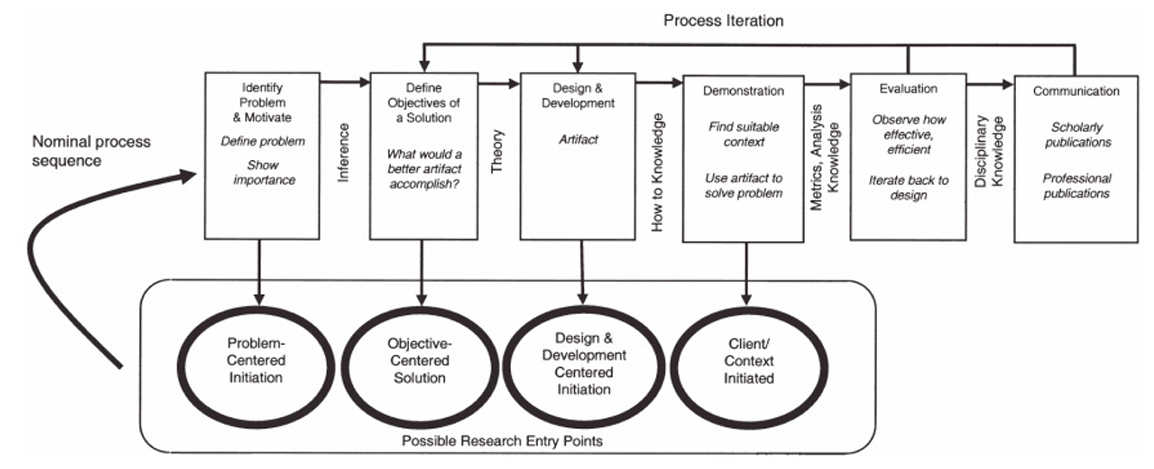
\includegraphics[width=1\linewidth]{ch1/dsr.png}
\caption{Metodologia DSR (\cite{peffers2007design})}
\label{fig:dsr}
\end{figure}

A metodologia DSR é composta por seis etapas, que se relacionam com o presente projeto da seguinte forma:

TODO retificar esta lista no fim do trabalho

\begin{itemize}
\item \textbf{Identificação e Motivação do Problema:} Foi realizada uma análise aprofundada dos desafios enfrentados pelas equipas de suporte técnico, nomeadamente a dificuldade em aceder rapidamente a informação precisa, a sobrecarga de pedidos repetitivos e a falta de padronização nas respostas.
\item \textbf{Definição de Objetivos para a Solução:} Com base nos problemas identificados, foram definidos objetivos claros, como a criação de uma solução baseada em RAG que melhore a eficiência do suporte técnico, assegure consistência nas respostas e possibilite a rastreabilidade das fontes de informação utilizadas.

\item \textbf{Desenho e Desenvolvimento:} Foi desenvolvido um protótipo funcional que integra uma arquitetura baseada em *Retrieval-Augmented Generation* com uma LLM, utilizando Spring AI. Este protótipo inclui também uma interface simples para interação e teste por parte dos utilizadores de suporte.

\item \textbf{Demonstração:} A solução foi aplicada a cenários simulados e reais de suporte técnico na área financeira, permitindo validar a sua aplicabilidade em tarefas como a resposta a incidentes, esclarecimento de dúvidas técnicas e recuperação de documentação normativa.

\item \textbf{Avaliação:} O sistema foi avaliado com base em testes de desempenho, testes unitários e de integração, bem como critérios de utilidade, precisão e conformidade com os requisitos regulatórios aplicáveis, incluindo os definidos pelo Banco Central Europeu.

\item \textbf{Comunicação:} Os resultados desta investigação foram documentados nesta dissertação e visam contribuir tanto para o avanço do conhecimento académico na área da IA aplicada ao suporte, como para a melhoria contínua de processos em contexto empresarial.

\end{itemize}




\section{Planeamento}


\section{Considerações Éticas}

Esta dissertação respeita o código de ética do Instituto Politécnico do Porto (\cite{codigo_2020}). Em conformidade com o Artigo 2.º, o trabalho observa princípios fundamentais como a legalidade, transparência, responsabilidade, confidencialidade, integridade e honestidade. Adicionalmente, a investigação cumpre as orientações previstas no Artigo 10.º, assegurando os mais elevados padrões de integridade científica, originalidade e verificabilidade.

O plágio e qualquer forma de má conduta académica são rigorosamente evitados, conforme estipulado no Artigo 6.º, nomeadamente na alínea 2.8, que exige a correta citação de todas as fontes. Quaisquer contributos de terceiros ou propriedade intelectual são devidamente creditados, em conformidade com o Artigo 10.º, alínea \textit{e}, que reforça a importância da citação precisa e da distinção relativamente a trabalhos anteriores.

Dado o carácter experimental desta investigação, apenas são utilizados conjuntos de dados e ferramentas com licenciamento explícito que permita a sua utilização académica. Além disso, e de acordo com o Artigo 10.º, alínea \textit{h}, eventuais conflitos de interesse e apoios externos são divulgados de forma transparente.

O conteúdo desta dissertação foi desenvolvido com diligência e rigor, garantindo a reprodutibilidade e a comunicação transparente dos resultados, conforme exigido pelo Artigo 10.º, alínea \textit{g}. Todos os métodos, fontes de dados e ferramentas utilizados nesta dissertação estão totalmente documentados e são publicamente acessíveis, contribuindo assim para uma comunicação científica aberta e transparente.

Por fim, todas as atividades foram realizadas com o devido respeito pelas obrigações éticas e legais no que respeita à privacidade de dados e à propriedade intelectual, conforme estipulado no Artigo 10.º, alínea 2a, e no Artigo 9.º, assegurando a segurança, bem-estar e os direitos de todos os participantes envolvidos.

\section{Estrutura do Documento}


% Chapter 2

\chapter{Key Concepts} % Main chapter title


%----------------------------------------------------------------------------------------

\section{Artificial Intelligence}

A inteligência artificial (IA) é um ramo cientifico da computação que se dedica ao desenvolvimento de sistemas capazes de executar tarefas que normalmente exigiriam inteligência humana.
Estes sistemas têm a capacidade de executar funções avançadas e analisar dados de grande escala a fim de gerar respostas precisas.  Baseado num conceito do filosofo do grego Aristoteles, a IA surgiu na década de 1950 por Allan Turing, onde o mesmo escreveu sobre a possibilidade de uma máquina pensar e imitar o comportamento humano inteligente. 
Atualmente a IA é aplicada em diversos setores, como na saúde através do diagnostico automatizado de doenças, no setor financeiro para análises de mercado e deteção de fraudes, entre outros. Recentemente a IA sofreu um "boom" tecnológico, com a corrida da IA generativa, sendo o seu componente-chave a fundação da OpenAI em 2015 e surgimento do ChatGPT em 2022, sistema este capaz de processar linguagem natural (NLP) e gerar respostas precisas e corretas sobre variados assuntos (https://hai.stanford.edu/news/ai-spring-four-takeaways-major-releases-foundation-models).

Dentro da IA existem diferentes sub-ramos cientificos, como:

\begin{itemize}
    \item Machine Learning (ML): Ensina computadores a aprender padrões a partir de dados através de redes neronais ou arvores de decisão;
    \item Deep Learning (DL): Sub-ramo do ML que faz uso de redes neronais para modelar a intrepertar padrões complexos;
    \item Processamento de linguagem natural (NLP): Intrepertação de linguagem natural humana.
    \item Visão computacional: Intrepertação de imagens e vídeos
\end{itemize}



\section{Machine Learning \& Deep Learning}

Diferença entre aprendizado de máquina e aprendizado profundo.
Como esses conceitos se relacionam com modelos de IA modernos.

\section{Large Language Models}

Os Large Language Models (LLMs) representam um avanço significativo na IA. Proposta pela Google em 2017, atualmente, Transformer é a arquitetura de DL mais explorada para esta componente. Os Transformers foram inicialmente desenvolvidos como melhoria das arquiteturas anteriores para a tradução automática, mas desde então têm encontrado muitas aplicações, como na visão computacional e NLP. Conduziram ao desenvolvimento de sistemas pré-treinados, tais como Generative Pre-trained Transformers (GPTs) and Bidirectional Encoder Representations from Transformers (BERT). Estes modelos são treinados através do paradigma Self-supervised learning (SSL), no qual aprendem representações úteis dos dados sem a necessidade de rótulos manuais. No SSL, o próprio modelo gera os seus rótulos a partir dos dados brutos, criando tarefas preditivas auxiliares chamadas pretext tasks. Masked Language Modeling é um exemplo de tarefa preditiva, utilizada pelo BERT, onde palavras altetórias são ocultadas em uma frase e o modelo aprende a prever as palavras corretas, isto no contexto de NLP. Em contraste o GPT faz uso do Casual Language Modeling onde o modelo prevê a próxima palavra numa sequência de texto, dado o contexto anterior.

\section{Retrieval-Augmented Generation}

Retrieval-Augmented Generation (RAG) é uma técnica que combina LLMs com um mecanismo de recuperação de informação externa. Enquanto que os LLMs apenas se baseiam em dados pré-treinados, o RAG recupera informação relevante de um contexto específico armazenado em base de dados ou documentos. 

Esta técnica conta com dois principais componentes: o  \textit{Retriever} e o  \textit{Generator}.

\begin{itemize}
    \item \textbf{Retriever}: Baseado na \textit{query} de \textit{input}, a função do \textit{Retriever} é percorrer o conhecimento disponível (p.e. base de dados vetoriais, documentos, fontes \textit{web}) e encontrar informação que vá de encontro a essa \textit{query}. Funciona como uma espécie de motor de busca e é essencial pois determina a relavância e qualidade da informação que será usada para gerar a resposta final. 
    \item \textbf{Generator}: O \textit{Generator} atua após o \textit{Retriever} ter feito a recuperação de informação relevante, juntando-a com a \textit{query} original para elaborar uma resposta contextualizada. O conhecimento pré-existente é tido em conta pelo o LLM permitindo que as respostas sejam mais inteligentes e informadas para o contexto em questão. 
\end{itemize}


RAG é atualmente usado, por exemplo, para suporte ao consumidor através da criação de Chatbots capazes de recuperar FAQs e o conhecimento do negócio de forma fácil. Gestão do conhecimento empresarial é outro exemplo de caso de uso, pois permite que os funcionários recuperarem e acedam a informação do contexto de trabalho de forma mais rápida. Este último caso de uso vai de encontro aos objetivos do presente projeto. 

TODO Incluir diagrama de arquitetura



\subsection{Prompt Templates}

São usados para guiar as repostas do modelo reproduzindo um PromptValue. Este é o resultado final da intrução a ser transmitida ao LLM assim que o input do utilizador for executado em cima do template. São importantes pois direcionam a instrução para a obtenção de respostas que vão de em contra ao objetivo da aplicação. 

\begin{lstlisting}[language=Python, caption={Using LangChain to create a prompt template}, label={lst:joke-prompt}]
from langchain_core.prompts import PromptTemplate

prompt_template = PromptTemplate.from_template("Tell me a joke about {topic}")

prompt_template.invoke({"topic": "cats"})
\end{lstlisting}

No contexto de uma aplicação para contar anedotas (\ref{lst:joke-prompt}), apenas com a especificação do tema da anedota, neste caso gatos, o template cria o PromptValue "Tell me a joke about cats"  a ser executado pelo LLM.


https://python.langchain.com/docs/concepts/prompt\_templates/


\subsection{Processo de indexação}

TODO entrar em mais detalhes do RAG pois isto é o core do projeto
TODO falar de mais componentes do RAG


\section{Bases de Dados Vetoriais}

Conceito de embeddings e busca vetorial.
Exemplos de ferramentas (FAISS, Weaviate, Pinecone).<
Importância da base vetorial no contexto do RAG.

\section{Aplicação ao Suporte Técnico}

Como esses conceitos são aplicáveis ao problema da dissertação.
Benefícios esperados da implementação.

% Chapter 3

\chapter{State of the Art} % Main chapter title
\label{chap:Chapter3} 

%----------------------------------------------------------------------------------------
\section{Methodology}

\subsection{Research Questions}

RQ1 - Como as frameworks ou bibliotecas disponíveis para desenvolvimento RAG se comparam em termos de arquitetura, flexibilidade e facilidade de utilização?

RQ2 - Quais são os desafios técnicos na implementação de uma solução baseada em RAG para suporte técnico?



RQ3 - Quais as melhores práticas para a indexação e recuperação de dados? 


RQ4 - Qual a LLM mais adequada para uso de RAG para suporte técnico? 




\subsection{Research Scope}

\subsection{Eligibility Criteria}


\subsection{Selection Process}

\subsection{Data Collection}

\section{Results and Analysis}



\subsection{RQ1 - Como as frameworks ou bibliotecas disponíveis para desenvolvimento RAG se comparam em termos de arquitetura, flexibilidade e facilidade de utilização?}

Antes de apresentar cada tecnologia, importa referir que as informações aqui descritas foram obtidas com base na respetiva documentação oficial disponível nos websites de cada projeto. Nesta análise, cada framework será avaliada segundo três critérios: (i) arquitetura, (ii) flexibilidade e (iii) facilidade de utilização. Adicionalmente, serão também consideradas as formas de integração com bases de dados externas (vector stores ou document stores), bem como o suporte e comunidade em torno de cada projeto.


\subsubsection{LangChain}


Fundada por Harrison Chase em 2022, LangChain é uma framework open-source para o desenvolvimento de aplicações que integram LLMs com fontes externas de dados e ferramentas de software. Está disponível em Python e JavaScript, oferecendo um ambiente centralizado e altamente extensível para construir soluções com LLMs de forma modular e reutilizável.

\paragraph{Arquitetura}

A arquitetura do LangChain é baseada no conceito de \textit{Chains}, que representam sequências de chamadas a LLMs e a outras ferramentas auxiliares. Estas \textit{Chains} podem ser compostas de forma modular, permitindo construir fluxos de execução complexos com facilidade.

Com a introdução do LangChain Expression Language (LCEL), passou a ser possível definir estas sequências de forma declarativa. O LCEL oferece diversos construtores prontos para uso, como:

\begin{itemize}
	\item \textit{create\_stuff\_documents\_chain}: Formata uma lista de documentos em um prompt para o LLM.
	\item \textit{create\_sql\_query\_chain}: Gera consultas SQL a partir linguagem natural.
	\item \textit{create\_history\_aware\_retrieve}: Utiliza o histórico de conversas para gerar consultas de busca mais precisas.
	\item \textit{create\_retrieval\_chain}: Integra recuperação de documentos relevantes com geração de respostas por LLM.
\end{itemize}


\paragraph{Flexibilidade}

LangChain é uma das frameworks mais flexíveis atualmente disponíveis. A sua estrutura modular permite criar soluções para diversos domínios — desde sistemas de chat com memória contextual até agentes com raciocínio multi-etapas e integração com APIs externas. Suporta LLMs de múltiplos fornecedores, incluindo:

\begin{itemize} \item OpenAI (via API Key) \item Cohere \item Anthropic (Claude) \item Modelos open-source (como LLaMA, Flan-T5, Mistral, etc.) via Hugging Face \end{itemize}

Os componentes podem ser combinados e substituídos livremente, o que torna o LangChain altamente adaptável a diferentes arquiteturas e necessidades de negócio.

\paragraph{Facilidade de utilização}

A curva de aprendizagem do LangChain pode ser ligeiramente acentuada devido à grande variedade de conceitos e componentes disponíveis. No entanto, a documentação é abrangente e inclui exemplos práticos, tutoriais e guias para casos de uso comuns.

O LCEL veio simplificar bastante o processo de criação de pipelines, ao permitir a definição declarativa de fluxos sem necessidade de escrita de código imperativo detalhado. Ainda assim, o domínio completo da framework pode exigir tempo, especialmente na fase de composição de agentes ou integração de ferramentas externas.

\paragraph{Integração com bases de dados vetoriais e document stores}

LangChain disponibiliza integração nativa com diversos sistemas de armazenamento de documentos, tanto tradicionais como vetoriais, tais como Elasticsearch e Weaviate, duas tecnologias open-source que permitem pesquisa vetorial, armazenamento de embeddings e indexação de documentos.

Estes sistemas são acedidos através de abstrações como \texttt{VectorStoreRetriever} e \texttt{DocumentLoaders}, que permitem a configuração e adaptação do processo de indexação e recuperação de informação de acordo com os requisitos específicos da aplicação.

\paragraph{Suporte e comunidade}

LangChain possui uma comunidade ativa e em crescimento, com elevado dinamismo no repositório GitHub, contanto com mais de cem mil estrelas. A empresa responsável pelo projeto, tem promovido o desenvolvimento contínuo da framework, bem como o lançamento de ferramentas complementares como o LangSmith, destinado à monitorização e depuração de aplicações baseadas em LLMs. Esta vitalidade comunitária traduz-se em documentação continuamente atualizada, partilha regular de boas práticas e integração frequente de contributos externos.


======================================================

https://www.ibm.com/think/topics/langchain
https://python.langchain.com/v0.1/docs/modules/chains/


======================================================



\subsubsection{Haystack}


Haystack é uma framework open-source desenvolvida pela empresa alemã Deepset, com o objetivo de facilitar a construção de pipelines baseadas em LLMs, especialmente para casos de uso como RAG, question answering, classificação, extração de informação e pesquisa semântica em documentos. A linguagem principal utilizada é Python. A primeira versão surgiu em 2020, tendo recentemente evoluído para a versão 2.0, com uma reformulação completa da sua arquitetura.

\paragraph{Arquitetura}

A principal inovação do Haystack 2.0 é a sua arquitetura orientada a componentes. Cada componente representa uma unidade funcional independente, com responsabilidade bem definida dentro de uma pipeline. Estes componentes são combinados de forma declarativa para formar pipelines personalizadas, robustas e escaláveis. Entre os tipos de componentes disponíveis encontram-se:

\begin{itemize} \item \textbf{Document Stores}: responsáveis por armazenar documentos e suportar tanto índices tradicionais quanto vetoriais. \item \textbf{Retrievers}: mecanismos de recuperação de informação, com suporte a métodos tradicionais como BM25 e a recuperação semântica com embeddings. \item \textbf{Rankers}: permitem reordenar os documentos recuperados com base em critérios de relevância mais refinados. \item \textbf{Generators}: utilizam LLMs para gerar respostas com base na informação recolhida. \item \textbf{Prompt Nodes}: enviam prompts configuráveis para modelos locais ou remotos. \item \textbf{Routers}: introduzem lógica condicional nas pipelines, facilitando a criação de fluxos adaptativos. \end{itemize}

As pipelines podem ser definidas em ficheiros YAML ou diretamente em Python, promovendo flexibilidade tanto para utilizadores técnicos como não técnicos.

\paragraph{Flexibilidade}

Haystack destaca-se pela sua grande flexibilidade. A arquitetura baseada em componentes independentes permite a substituição e reconfiguração de cada etapa do fluxo de processamento, facilitando a adaptação a diferentes domínios, fontes de dados e estratégias de interação com LLMs. Os desenvolvedores podem ainda combinar múltiplos retrievers, utilizar lógica condicional com routers e integrar diversos serviços externos com relativa facilidade.

\paragraph{Facilidade de utilização}

A curva de aprendizagem do Haystack pode ser moderada, especialmente para utilizadores que não estejam familiarizados com conceitos como pipelines declarativas ou integração com serviços externos. No entanto, a documentação oficial é bastante completa e a existência de pipelines pré-configuradas — como a \texttt{PredefinedPipeline.INDEXING} e a \texttt{PredefinedPipeline.RAG} — facilita bastante o início do desenvolvimento. Estas permitem, respetivamente, indexar documentos e realizar tarefas de RAG com configuração mínima.

\paragraph{Integração com bases de dados vetoriais/document stores}

Haystack oferece suporte nativo a várias tecnologias de armazenamento de documentos, como Elasticsearch e Weaviate, referidos anteriormente. Em ambiente de desenvolvimento, o Haystack oferece o InMemoryDocumentStore, uma opção lightweight que armazena os documentos diretamente em memória, sendo ideal para testes.

\paragraph{Suporte e comunidade}

Haystack possui uma comunidade ativa. O repositório oficial no GitHub conta com mais de vinte mil estrelas (TODO referencia github), issues frequentemente respondidas, e releases regulares. A documentação é extensa, com guias, tutoriais e exemplos práticos.


======================================================

https://medium.com/aimonks/haystack-an-alternative-to-langchain-carrying-llms-bf7c515c9a7e
https://haystack.deepset.ai/overview/intro
https://docs.haystack.deepset.ai/docs/pipeline-templates



\subsubsection{LlamaIndex}

TODO



\subsubsection{Spring AI}


Spring AI é uma framework recente, disponibilizada publicamente no início de 2024, com o objetivo de simplificar o desenvolvimento de aplicações baseadas em inteligência artificial, especialmente no ecossistema Java. Inspirado por projetos como LangChain e LlamaIndex, o Spring AI surge como uma extensão natural do ecossistema Spring, promovendo a integração de LLMs em aplicações corporativas de forma modular, acessível e escalável.

\paragraph{Arquitetura}

A arquitetura do Spring AI é orientada a componentes e organizada em torno do conceito de \emph{Advisors}, responsáveis por encapsular diferentes estratégias de interação com LLMs e bases de dados vetoriais. A framework disponibiliza dois tipos principais de \textit{advisors} para fluxos RAG:

\begin{itemize} 
        \item \textbf{QuestionAnswerAdvisor}: foca-se na recuperação exata de informação a partir de dados externos, construindo respostas exclusivamente com base nos documentos recuperados da base vetorial. 
        \item \textbf{RetrievalAugmentationAdvisor}: combina a informação externa com o conhecimento prévio embutido no modelo base, permitindo uma resposta enriquecida e mais flexível. 
\end{itemize}

A comunicação com estes componentes é configurada programaticamente através da API do Spring AI, possibilitando a definição de parâmetros como o limiar de similaridade na pesquisa.

Adicionalmente, a framework estrutura os fluxos de processamento em módulos reutilizáveis, entre os quais se destacam: 
\begin{itemize} 
        \item \emph{Document Reader Modules} - para leitura e preparação de documentos; 
        \item \emph{Embedding Modules} - para geração de vetores a partir de texto; \item \emph{Retriever Modules} - para pesquisa em bases vetoriais; 
        \item \emph{LLM Modules} - para interação com o modelo de linguagem. 
\end{itemize}

Esta abordagem modular facilita a composição e manutenção de pipelines RAG personalizadas.

\paragraph{Flexibilidade}

Apesar de ser uma framework emergente, o Spring AI apresenta uma estrutura suficientemente flexível para acomodar diversos casos de uso. A separação clara entre módulos permite que cada fase do pipeline seja configurada ou substituída conforme os requisitos específicos da aplicação.

A framework suporta múltiplos provedores de LLMs, incluindo OpenAI, Hugging Face, Mistral e Cohere, entre outros, com mecanismos de autenticação e configuração standard através do ecossistema Spring.

Por estar profundamente integrado com o ecossistema Spring, a framework beneficia de recursos como injeção de dependências, configuração centralizada, gestão de contexto e integração com outras soluções do universo Spring Boot, o que a torna especialmente atrativa para ambientes corporativos baseados em Java.

\paragraph{Facilidade de utilização}

Um dos principais objetivos do Spring AI é tornar a utilização de LLMs mais acessível a programadores do ecossistema Java. A framework herda a familiaridade e consistência do paradigma Spring, oferecendo uma experiência previsível e bem documentada.

Os \textit{advisors} e módulos podem ser facilmente instanciados e configurados, sendo suportados por exemplos concisos e tutoriais disponíveis na documentação oficial. A integração com ferramentas padrão do Spring (como o Spring Boot Actuator ou o Spring Configuration) facilita a observabilidade e a gestão de parâmetros em ambientes de produção.

Contudo, como se trata de uma framework ainda em evolução, podem existir limitações ao nível de abstrações mais avançadas quando comparada com alternativas mais consolidadas no ecossistema Python.

\paragraph{Integração com bases de dados vetoriais e document stores}

O Spring AI oferece integração nativa com várias bases de dados vetoriais, através da abstração \texttt{VectorStore}. Atualmente, estão disponíveis conectores para:

\begin{itemize} \item \textbf{FAISS} \item \textbf{Qdrant} \item \textbf{Pinecone} \item \textbf{Weaviate} \end{itemize}

Estes armazenamentos vetoriais podem ser utilizados diretamente nos módulos de recuperação, com suporte para parâmetros como o número de documentos a recuperar e o grau de similaridade exigido.

A framework prevê ainda a evolução para incluir mecanismos mais elaborados de pré-processamento de documentos, nomeadamente para segmentação, limpeza e enriquecimento semântico dos conteúdos.

\paragraph{Suporte e comunidade}

Dado o seu lançamento recente, a comunidade do Spring AI ainda se encontra em crescimento. No entanto, beneficia do forte ecossistema da Spring Framework e da extensa base de utilizadores da comunidade Java. O projeto é mantido pela equipa oficial da Spring, o que garante qualidade no design, documentação consistente e ciclos de lançamento regulares.

A documentação oficial cobre os principais casos de uso, e já existem exemplos práticos disponíveis em repositórios públicos que demonstram a aplicação da framework em pipelines RAG.


\subsubsection{Comparação resumo entre tecnologias}


Para resumir, na Tabela \ref{tab:tec-comp} estão descritos os principais pontos de comparação entre as diferentes tecnologias analisadas. 

\begin{table}[H]
        \centering
        \caption{Comparação entre tecnologias RAG}
        \label{tab:tec-comp}
        \renewcommand{\arraystretch}{1.2}
        \begin{tabularx}{\textwidth}{|X|X|X|X|X|X|}
        \hline
        \textbf{Ferramenta} & \textbf{Arquitetura} & \textbf{Flexibilidade} & \textbf{Facilidade de utilização} & \textbf{Integração com bases vetoriais / document stores} & \textbf{Suporte, comunidade e documentação} \\
        \hline
        \textbf{LangChain} & Orquestração modular e declarativa & Elevada & Intermédia &  FAISS, Pinecone, Chroma, Redis, Weaviate, Qdrant. & Comunidade / Suporte \textbf{++} ; Documentação extensa \\
        \hline
        \textbf{Haystack} & Arquitetura orientada a componentes & Elevada & Intermédia a alta & Suporte robusto com "Document Stores" como Elasticsearch, Qdrant, Weaviate; suportando indexação vetorial e tradicional. & Comunidade / Suporte \textbf{+++} ; Documentação extensa \\
        \hline
        \textbf{Spring AI} & Arquitetura modular; integração com o ecossistema Spring. & Moderada a elevada & Alta para programadores Java & FAISS, Qdrant, Pinecone, Weaviate; integração através de "VectorStore". & Comunidade / Suporte \textbf{+} ; Documentação em crescimento  \\
        \hline
        \end{tabularx}
    \end{table}

Em termos de arquitetura as tecnologias são semelhantes em alguns principios gerais, mas diferem na forma como organizam os componentes. A LangChain usa o conceito de chains e agents que permite encadear multiplos passos de forma declarativa. Já a Haystack possui um arquitetura orientada a componentes reutilizáveis. Na Spring AI a arquitetura é modular e integrada no ecossistema Sprint Boot com foco para desenvolvedores Java, usando abstrações típicas do Spring. 


No que diz respeito à flexibilidade, LangChain e Haystack oferecem maior capacidade de personalização, com suporte a múltiplas configurações e integrações. O Spring AI, apesar de mais recente, apresenta uma modularidade sólida, embora mais orientada a padrões corporativos Java.

Em termos de facilidade de utilização, o Spring AI proporciona uma curva de aprendizagem mais suave para programadores familiarizados com Spring Boot. A Haystack combina flexibilidade com pipelines pré-configuradas, ao passo que a LangChain, apesar de poderosa, exige maior domínio técnico para compor soluções complexas.

Todas as ferramentas analisadas oferecem integração com sistemas de armazenamento vetorial da atualidade, como FAISS, Qdrant e Weaviate. O suporte é robusto e adaptável em todas, com destaque para a abstração VectorStore no Spring AI e a diversidade de conectores nativos no Haystack.

Por fim, no que respeita a suporte e comunidade, LangChain e Haystack apresentam ecossistemas consolidados, com documentação extensa, comunidades ativas e evolução contínua — refletido na Tabela \ref{tab:tec-comp} com os níveis \textbf{++} e \textbf{+++}, respetivamente. O Spring AI, embora ainda em fase de maturação, conta com documentação estruturada e o respaldo da comunidade Spring, o que lhe confere um nível \textbf{+} na escala adotada, indicando um bom ponto de partida com potencial de crescimento acelerado.

        

\subsection{RQ2- Quais são os desafios técnicos na implementação de uma solução baseada em RAG para suporte técnico?}

Existem diversos desafios técnicos na implementação de uma solução RAG para suporte técnico, tais como para a indexação e recuperação de dados, a integração com sistemas existentes no sentido de alimentação do conhecimento e precisão e relevância das respostas. 

\subsubsection{Indexação, recuperação e relevância das respostas}

A eficiência do RAG depende da capacidade de recuperar documentação relevante. No contexto de suporte técnico, a recuperação necessita ser precisa para fornecer soluções corretas o que é desafiador devido à complexidade e especificidade da documentação \parencite{ToroIsaza2024}.


No que toca recuperação por similaridades semanticas, \cite{soman2024observations} refere que o uso de embeddings para chunks de texto grandes (> 200 palavras) resulta em valores de similaridade artificialmente altos. Isso sugere que, mesmo quando as frases não são semanticamente parecidas, o modelo acha que são, apenas por serem longas. Contudo, documentação que usa grande número de abreviações e paragrafos para um tópico tornanam as obeservações mais relevantes. Além disso, concluiu-se palavras-chave mais próximas do começo de de uma frase são recuperadas com maior precisão.

Adicionalmente, estudos recentes revelam que sistemas RAG apresentam dificuldades significativas quando aplicados em ambientes empresariais. \textcite{RAGDoesNotWork2024} demonstram que, mesmo quando a resposta correta está presente no contexto, o sistema frequentemente falha em recuperá-la. Isso ocorre, em parte, devido ao desajuste entre a estrutura dos documentos técnicos (como FAQs, procedimentos, logs, etc.) e as estratégias tradicionais de segmentação em chunks.

Essa falha é confirmada por \textcite{SevenPoints2024}, que identificaram múltiplos pontos críticos no funcionamento de sistemas RAG, incluindo:

\begin{itemize}
    \item Falta de conteúdo: Quando a informação necessária não está no contexto, o sistema pode responder com conteúdos enganosos, sugerindo que sabe a resposta mesmo sem dados de apoio.
    \item Fraca classificação da documentação: Mesmo com a informação presente no contexto, ela pode não ser corretamente classificada e consequentemente não recuperada. 
 \item Informação não extraida: Caso haja informações contraditórias no contexto, o retriever pode apresentar falhas.
  \item Especificidade incorreta: O sistema pode gerar respostas muito vagas ou excessivamente específicas sem compreender especificamente o que foi solicitado.
\end{itemize}

Diversas técnicas de Finetunning podem ser utilizadas para contornar estas situações.

TODO melhorar daqui para baixo
Contextos maiores geram respostas mais precisas. A inclusão de metadados, como o nome do ficheiro e número do chunk, melhora a interpretação da informação recuperada. Modelos de embeddings open source também se mostram eficazes, especialmente em textos curtos. Para garantir resultados robustos, é essencial calibrar cuidadosamente o pipeline RAG — incluindo chunking, embeddings, recuperação e consolidação — além de manter uma monitorização contínua, dado que o sistema lida com entradas desconhecidas em tempo real.



\subsubsection{Integração com Sistemas Existentes}




https://arxiv.org/pdf/2409.13707

https://arxiv.org/pdf/2404.00657


\section{Related Work}

TODO incluir isto?: Embora o foco desta dissertação seja a aplicação de RAG em contextos de suporte técnico, são também analisados trabalhos em domínios adjacentes quando estes oferecem contributos relevantes em termos de arquitetura, avaliação ou boas práticas.

\subsection{RAG chatbot para a OptiMicro Technologies}

A OptiMicro, empresa de software Canadiana, decidiu apostar no desenvolvimento de um chatbot utilizando RAG para melhorar o seu serviço de apoio técnico da empresa, mais especificamente no seu serviço DentalWare.

O software foi desenvolvido através de uma plataforma lowcode denominada Flowise AI e a sua arquitetura consistiu em três fases principais: indexação, recuperação e geração. Na fase de indexação, foram utilizados registos de suporte técnico e manuais do software DentalWare, segmentados em chunks de texto. Os dados foram convertidos em vetores através do modelo all-MiniLM-L6-v2, acedido via API da HuggingFace, e armazenados numa base de dados vetorial Pinecone, escolhida pela sua elevada performance. Na etapa de recuperação, a query do utilizador é embedded com o mesmo modelo e comparada com os vetores indexados, sendo selecionados os segmentos mais relevantes. Por fim, a resposta é gerada com o modelo LLaMA 2 (7B), executado localmente via Ollama. 

Esta arquitetura encontra-se descrita no diagrama da Figura \ref{fig:opti-micro-arch}, onde é possível verificar de que forma os componentes se relacionam. É de notar que foram utilizados dois documentos como fonte de informação externa definidos de forma estática, tornando o software um pouco restrito.

\begin{figure}[H]
        \centering
        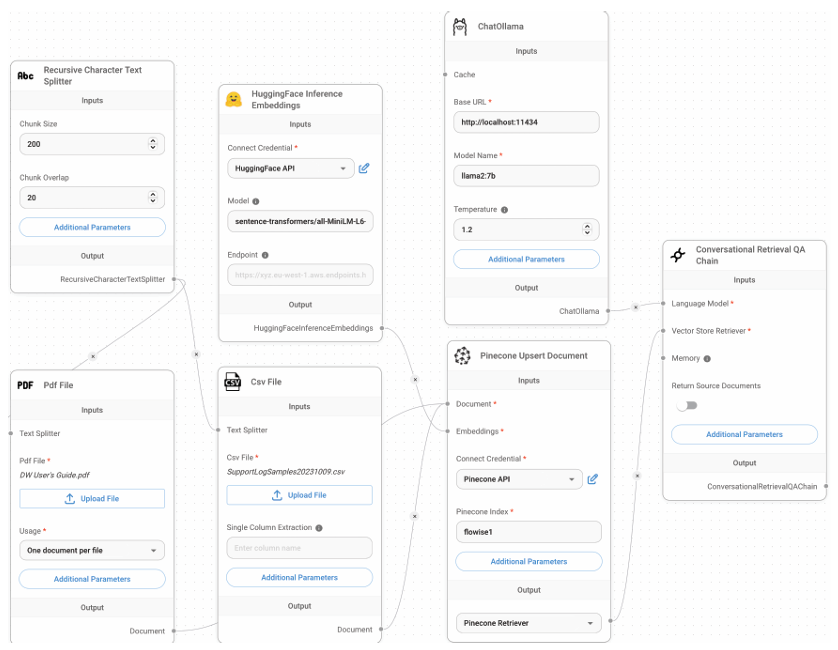
\includegraphics[width=1\linewidth]{ch3/assets/optimicro-arch.png}
        \caption{Arquitetura do chatbot RAG da OptiMircro \parencite{lee2024development}}
        \label{fig:opti-micro-arch}
\end{figure}


Para avaliar o desempenho do chatbot, foram utilizadas 75 questões reais relacionadas com suporte técnico ao software DentalWare. As respostas geradas por este chatbot foram comparadas com as de um chatbot LLM genérico, tendo ambas sido avaliadas com base nos critérios de ROUGE (ROUGE-1, ROUGE-2 e ROUGE-L) e por humanos da OptiMicro. Os resultados demonstraram que o chatbot RAG obteve melhores pontuações em todas as métricas ROUGE, destacando-se com aumentos de 38\%, 18\% e 40\%, respetivamente, face ao modelo genérico, o que evidencia uma maior fidelidade aos conteúdos técnicos. Na avaliação humana, o chatbot RAG obteve 20 respostas classificadas como boas, 18 como razoáveis e apenas 2 como fracas, enquanto o LLM genérico apresentou apenas 3 boas respostas e 2 razoáveis, totalizando 70 respostas consideradas fracas. Estes resultados confirmam a superioridade do modelo RAG no contexto de apoio técnico, pela sua capacidade de gerar respostas mais relevantes e alinhadas com os dados específicos da empresa.



TODO ponto negativa deste software: não foi implementado mecanismo para atualizar automaticamente a base de dados vetorial consoante updates na documentação


\subsection{Retrieval Augmented Generation-Based Incident Resolution Recommendation System for IT Support} 

TODO discutir este artigo
ficheiro IT SUPPORT RECOMENDATION.pdf nas transferencias


\subsection{Fabula}

ficheiro fabula.pdf nas transferencias
não é relacionado com IT support mas se calhar é interessante incluir para demonstrar outro caso de uso do RAG e pode dar algum insight util




%\input{ch4/chapter4}
%\input{ch5/chapter5}


%----------------------------------------------------------------------------------------
%	BIBLIOGRAPHY
%----------------------------------------------------------------------------------------

\printbibliography[heading=bibintoc]

%----------------------------------------------------------------------------------------
%	THESIS CONTENT - APPENDICES
%----------------------------------------------------------------------------------------
% Include the appendices of the thesis as separate files from the Appendices folder
% Uncomment the lines as you write the Appendices
\begin{appendices}

% Appendix A

\chapter{Appendix Title Here} % Main appendix title

\label{AppendixA} % For referencing this appendix elsewhere, use \ref{AppendixA}

Write your Appendix content here.
%\input{appendices/appendixB}
%\input{appendices/appendixC}

\end{appendices}
%----------------------------------------------------------------------------------------

\end{document}
